\documentclass{beamer}
\usepackage{amsfonts}
\usepackage{amsmath}
\usepackage{amssymb}
\usepackage[latin1]{inputenc}                                 
\usepackage{color}                                            
\usepackage{array}                                            
\usepackage{longtable}                                        
\usepackage{calc}                                             
\usepackage{multirow}                                         
\usepackage{hhline}                                           
\usepackage{ifthen}
\def\inputGnumericTable{}
\usepackage{graphicx}
\graphicspath{ {./figures/} }

\usetheme{CambridgeUS}

\title{\textbf{AI1110 \\ Assignment 8} }
\author{\textbf{Dondapati Chandrahas Reddy}\\\textbf{AI21BTECH11010}}

\begin{document}
	

\begin{frame}
	\titlepage 
\end{frame}


\section{Papoulis Example 5.2}
\begin{frame}{Question (Papoulis Example 5.2)}

We shall express the cumulative distribution function $F_Y(y)$ of the random yariable $Y = X^2$ in
terms of the cumulative distribution function $F_X(x)$ of the random variable $X$.

\end{frame}


\begin{frame}{Solution}
	\textbf{Case 1:} $y \geq 0$\\
	\begin{align}
		F_Y(y) &= P(Y < y)\\[1ex]
		&=P(X^2 < y)\\[1ex]
		&=P(-\sqrt{y} \leq X \leq \sqrt{y})\\[1ex]
		&=F_X(\sqrt{y})-F_X(-\sqrt{y})
	\end{align}
\end{frame}


\begin{frame}{Solution(Contd.)}
	\textbf{Case 2:} $y < 0$\\[1em]
	There are no values of $X$ such that $X^2 < y$\\[1ex]
	Hence $F_Y(y) = P(\emptyset) = 0$
\end{frame}


\begin{frame}{Example}
	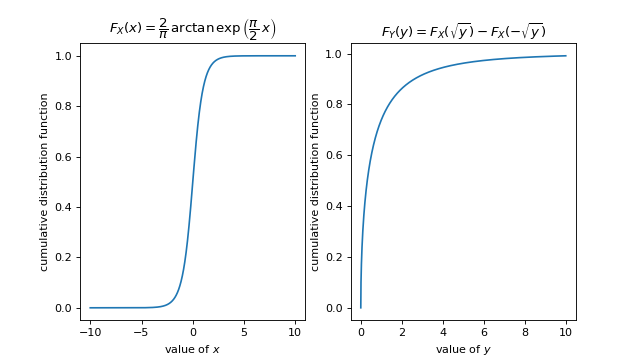
\includegraphics[scale=0.595]{fig1.png}
	Example: Let $y =4$ ,$F_Y(4) = 0.945, F_X(2) = 0.9725, F_Y(-2) = 0.0275$\\
	Hence Verified.
\end{frame}

\end{document}